\documentclass[a4paper, 12pt]{article}

\usepackage[T1]{fontenc}
\usepackage[utf8]{inputenc}
%\usepackage{lmodern}
%\usepackage{hyperref}
\usepackage{nohyperref} % This makes hyperref commands do nothing without errors
\usepackage{url}
\usepackage{graphicx}
\usepackage{seqsplit} 
\usepackage{varioref} % for vref
\usepackage{tabularx}
\usepackage{tabulary}
\usepackage{enumerate}
\usepackage[acronym]{glossaries}

\newacronym{nhs}{NHS}{National Health Service}
\newacronym{tds}{TDS}{Traffic Distribution Software}
\newacronym{candc}{C\&C}{Command-and-Control}

\makeglossaries

% Variables
\renewcommand{\title}{Ransomware: A systematic overview}
\renewcommand{\author}{Jan Schlenker}

\newcommand{\tabitem}{~~\llap{\textbullet}~~}

\setlength{\parindent}{0pt} % no indent after figure
\setlength{\skip\footins}{1cm} % indent before footnote

% ******************** BEGIN OF DOCUMENT ********************
\begin{document}

\begin{titlepage}

\newcommand{\HRule}{\rule{\linewidth}{0.5mm}} % Defines a new command for the horizontal lines, change thickness here

\center % Center everything on the page
 
%----------------------------------------------------------------------------------------
%	HEADING SECTIONS
%----------------------------------------------------------------------------------------

\textsc{\LARGE University of Innsbruck}\\[1.5cm] % Name of your university/college
\textsc{\Large Seminar Work}\\[0.5cm] % Major heading such as course name
\textsc{\large Master Seminar 2 (703606 SE/2)}\\[0.5cm] % Minor heading such as course title

%----------------------------------------------------------------------------------------
%	TITLE SECTION
%----------------------------------------------------------------------------------------

\HRule \\[0.4cm]
{ \huge \bfseries \title}\\[0.4cm] % Title of your document
\HRule \\[1.5cm]
 
%----------------------------------------------------------------------------------------
%	AUTHOR SECTION
%----------------------------------------------------------------------------------------

\begin{center}
\begin{tabular}{l l}
Author: & \author \\
Supervisor: & Christian Sillaber \& Clemens Sauerwein \\
Semester: & SS 2016/2017
\end{tabular}
\end{center}

% If you don't want a supervisor, uncomment the two lines below and remove the section above
%\Large \emph{Author:}\\
%John \textsc{Smith}\\[3cm] % Your name

%----------------------------------------------------------------------------------------
%	DATE SECTION
%----------------------------------------------------------------------------------------

%{\large \today}\\[3cm] % Date, change the \today to a set date if you want to be precise

%----------------------------------------------------------------------------------------
%	LOGO SECTION
%----------------------------------------------------------------------------------------

%\includegraphics{Logo}\\[1cm] % Include a department/university logo - this will require the graphicx package
 
%----------------------------------------------------------------------------------------

\vfill % Fill the rest of the page with whitespace

\end{titlepage}

%\include{01_abstract}

\tableofcontents
\newpage

\printglossary[title=List of Acronyms, type=\acronymtype]
\listoffigures
\listoftables

\section{Introduction}

Ransomware is one of the biggest cybercrime threats of our days, both for organizations and individuals. This was again demonstrated by the recent global attack of the WannaCry trojan \cite{Symantec2017} shown in figure \ref{fig:wanna_cry}, where more than 230000 computers in 150 different countries got infected. The attack also showed that there is often still no other way for infected victims than paying the ransom, if they want to get their data back and have no sufficient Backups. Precautions like regular security updates can help to avoid the damage, but there is no waterproof solution and people working with crucial data need to be educated about the topic. Among others, the \gls{nhs} faced huge troubles through WannaCry \cite{Martin2017}, which exemplifies that wallets can be affected by ransomware as well as health conditions.

\begin{figure}[htbp]
  \begin{center}
    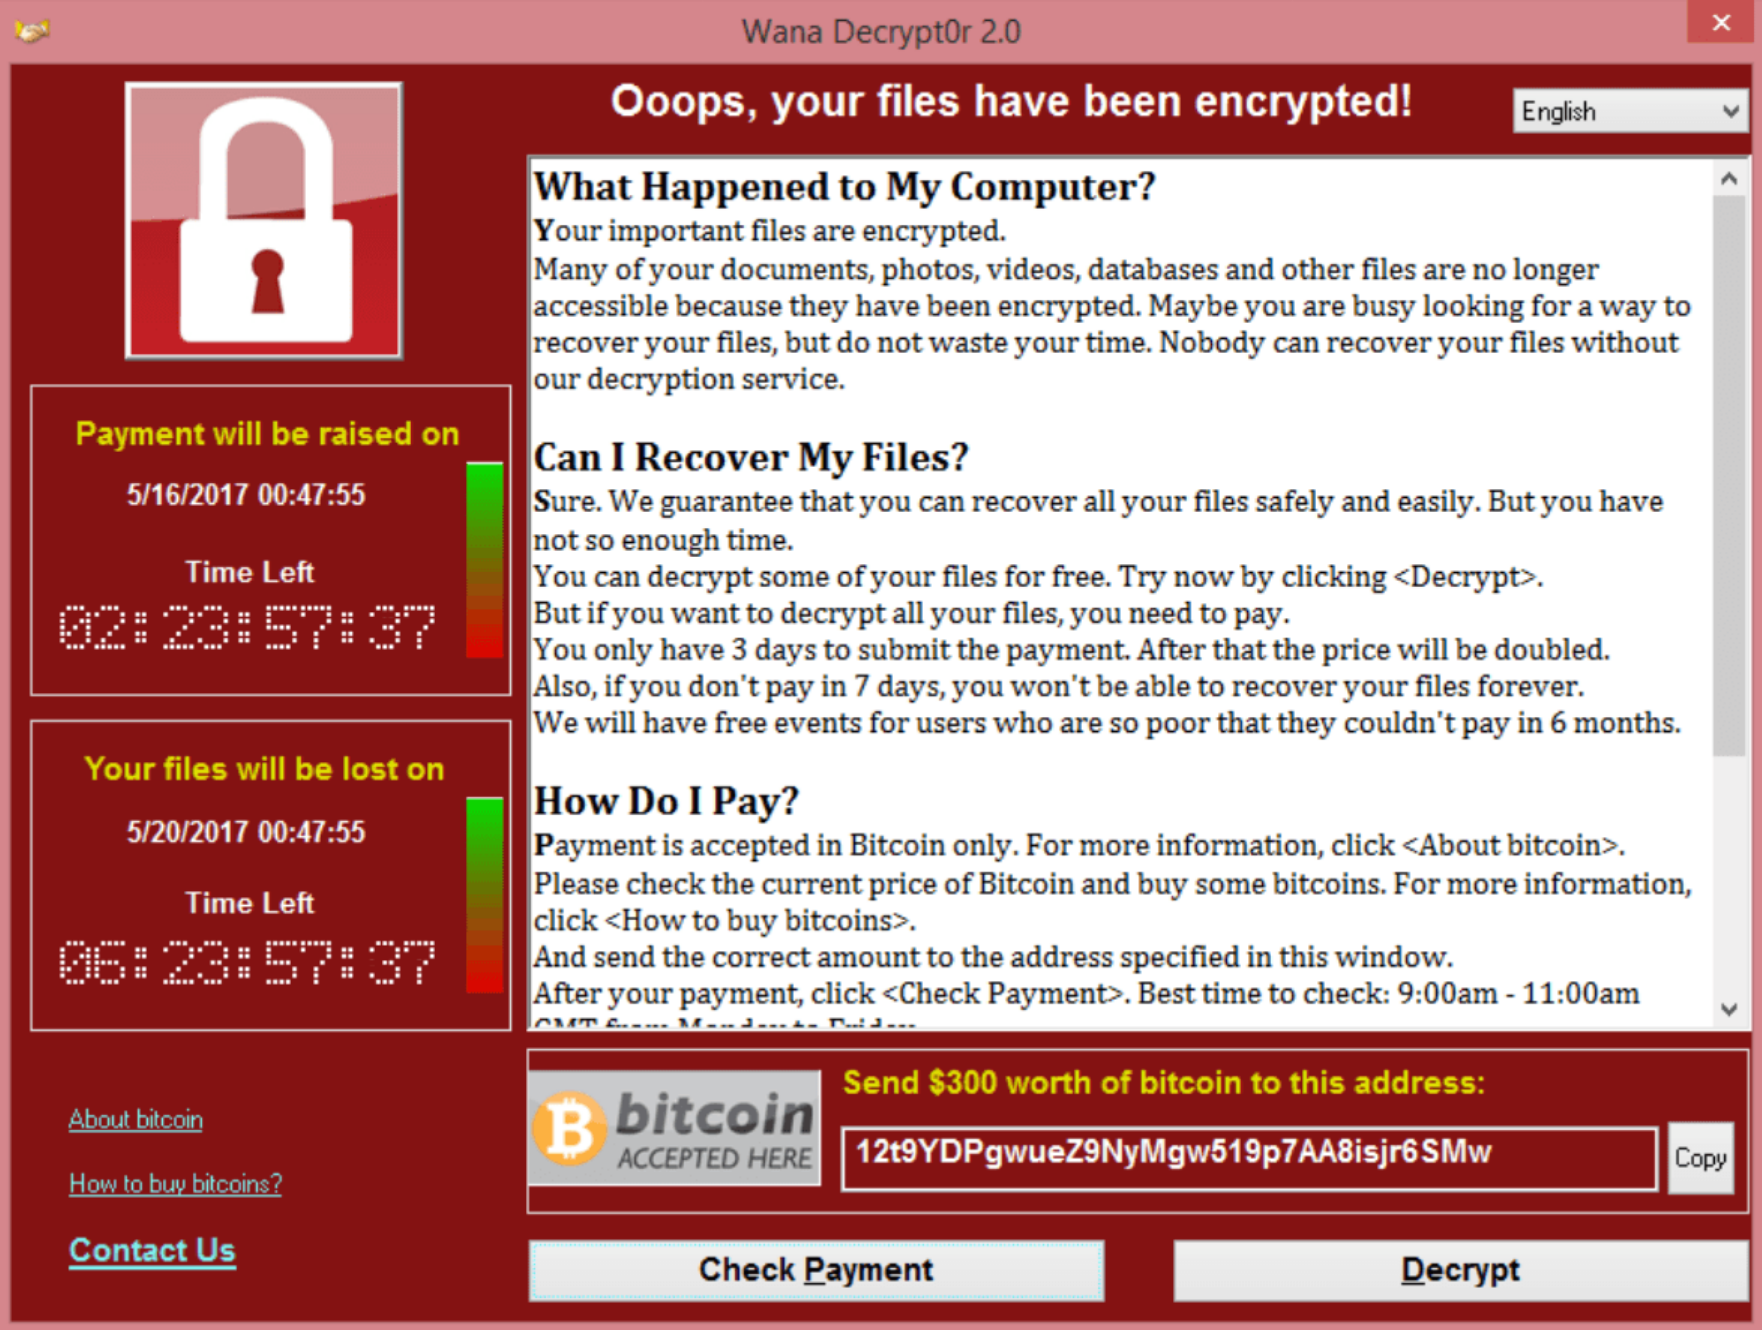
\includegraphics[width=0.8\textwidth]{images/wanna_cry.png}
    \caption{WannaCry Ransomware}
    \label{fig:wanna_cry}
  \end{center}
\end{figure}

This seminar work focuses on giving an overview of ransomware.
%TODO

\section{What is Ransomware?}

Ransomware in general is a malicious software, that denies access to the files of the victim or/and threatens to publish them. Most of the time it is distinguished by researchers into 2 major types:

\begin{description}
\item[File lockers:] The most common ransomware type, also known as ``crypto trojan'' or ``crypto ransomware''. Here the files of the victim are usually encrypted and the attacker demands the ransom for the decryption. Some variants do not encrypt the files but deny the access to the files in some other way, for example by putting them into a password protected archive \cite{Symantec2017a}.
  
\item[Screen lockers:] Here the victims access to its system is denied, mostly by changing the password or the pin. In this case the attacker demands the ransom for the new authentication code.
\end{description}

Pure screen lockers are not as dangerous as file lockers, because the (personal) files of the victim are not touched and can be recovered by accessing the harddrive from another system. However, file and screen lockers can be combined, which would prevent this recovering technique.\\
\\
Some sources name ``Leakware'' also known as ``Doxware'' as a third ransomware type \cite{Upadhaya2017}, where the attacker demands the ransom for not publishing the data of the victim. Companies can be targets, which do not want to share crucial data with their competitors, but also individuals, which for example have intimate photos on their device. Likewise this type can be combined with screen and file lockers.\\
\\
In contrast to other malware, ransomware reveals itself to the victim at some point (e.g. when the files are encrypted). Traditional malware rather aims to achieve stealth for collecting banking credentials or keystrokes without raising suspicion \cite{Kirda2017}. Ransomware on the other hand wants to get the attention of the victim to demand the ransom.

\section{How does it work?}
\subsection{Attack overview}
\label{subsec:attack_overview}

As mentioned file lockers are the most common ransomware type. An exemplified attack scenario is shown in Figure \ref{fig:attack_scenario}.

\begin{figure}[htbp]
  \begin{center}
    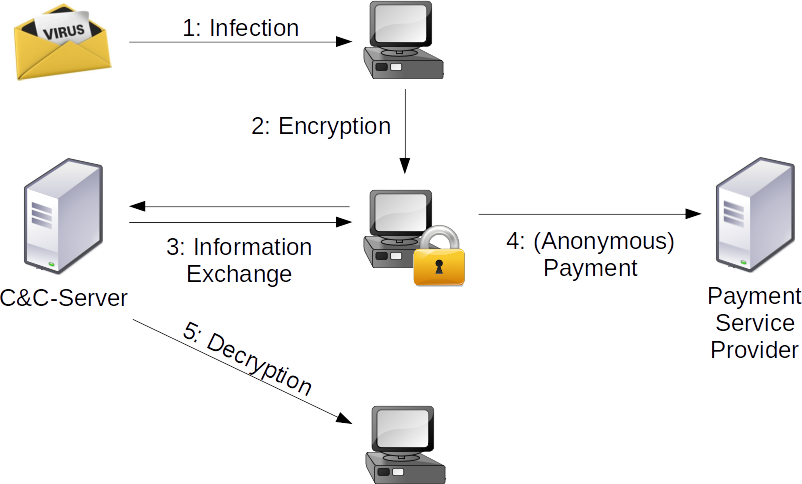
\includegraphics[width=0.8\textwidth]{images/attack_scenario.png}
    \caption{Attack scenario with file lockers}
    \label{fig:attack_scenario}
  \end{center}
\end{figure}

\begin{enumerate}
\item The device of the victim gets infected. Most of the time this happens via mail \cite{OstermanResearch2016}, where it either contains a link to a malicious software or the malicious software is attached directly. \glspl{tds}, malvertisement and social engineering are also used sometimes. Many ransomware variants further infect external storages and devices in the same network.
\item The files of the victim are encrypted. Normally the virus searches for files with specific file endings, which likely are important for the user. For example image file endings like .png and .jpg, as well as Microsoft Word file endings like .doc and .docx are often used. For the encryption itself in recent years well established cryptocraphic standards like AES-128 CBC. The encryption will be discussed in more detail in subsection \ref{subsec:encryption_overview}.
\item The information exchange with the \gls{candc} server. This servers are used to control botnets, but they are also used to communicate with infected devices of ransomware. Often \gls{candc} servers are located in countries with not so stringend law enforcement, so that they can stay alive as long as possible to exchange information with existing and new victims. Usually an unique identifier for every infected device is stored on the server as well as information about the device itself (e.g. number of infected files, infection time etc.). Making contact with a \gls{candc} server can also happen before the encryption, so that unique public/private key pairs are generated for every infected machine.
\item The victim pays the ransom to a payment provider. With the upsurge of crypto currencies like Bitcoin and networks like Tor, it is easier for attackers to stay anonymous when receiving the payment\cite{Liao2016}.
\item The encrypted files of the victim are decrypted. The attacker checks the payment beforehand and initializes the decryption. Therefore the key for the decryption is send to the victim. Some ransomware variants decrypt the files on the \gls{candc} server and send the decrypted files to the victim. Of course there is no gurantee for the victim, that the files are decrypted at all.
\end{enumerate}

As mentioned before this is only an examplified attack scenario. There exist many different variants with different scenarios.

\pagebreak
\subsection{Enryption overview}
\label{subsec:encryption_overview}

In recent years ransomware developers have used both asymmetric and symmetric cryptographic technologies. Figure \ref{fig:encryption_overview} illustrates when these technologies are used.

\begin{figure}[htbp]
  \begin{center}
    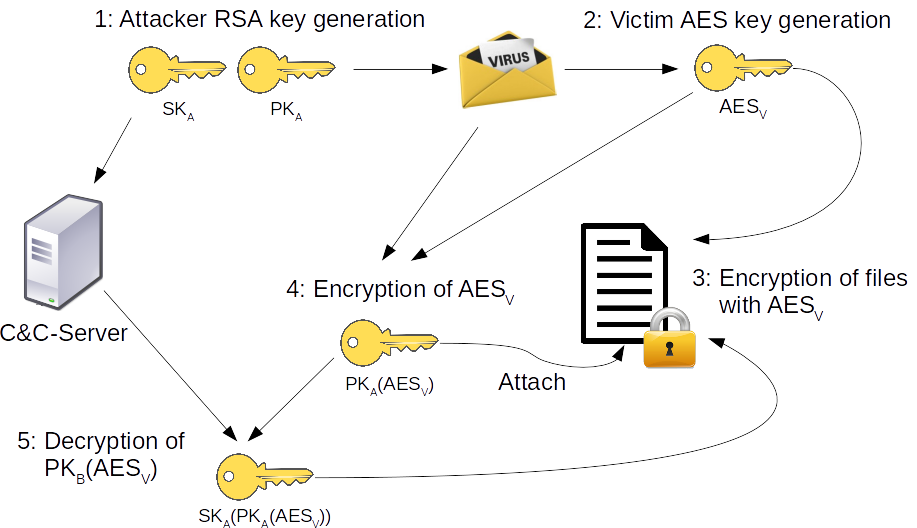
\includegraphics[width=0.8\textwidth]{images/encryption_overview.png}
    \caption{Ransomware encryption overview}
    \label{fig:encryption_overview}
  \end{center}
\end{figure}

\begin{enumerate}
\item The attacker generates and RSA key pair. He stores the secret key $SK_A$ on a \gls{candc} server and includes the public key $PK_A$ in the ransomware. Some ransomware variants create multiple of these key pairs.
\item On the victims device an AES session key $AES_V$ is generated. The generation is triggered by the ransomware on the infected device.
\item The files of the victim are encrypted with the AES session key $AES_V$.
\item The AES session key $AES_V$ is encrypted with the RSA public key $PK_A$. This new key $PK_A(AES_V))$ is often attached to the encrypted files, so that the {candc} server later can decrypt the files by only receiving the files. The AES session key $AES_V$ itself is safely deleted.
\item The key $PK_A(AES_V))$ is decrypted with the secret key $SK_A$. When a decrypted file arrives at the \gls{candc} server, it uses the stored secret key $SK_A$ to decrypt the attached key $PK_A(AES_V)$.\\
With $SK_A(PK_A(AES_V))$ the original AES key $AES_V$ can be restored.
\item The files can be decrypted with the key $AES_V$.
\end{enumerate}


\bibliographystyle{unsrt}
\bibliography{bibliography}

\section*{Declaration of Authorship}

\noindent I, \emph{\author}, declare that this seminar work titled \emph{\title} and the work presented in it are my own. I confirm that:

\begin{itemize} 
\item Where I have consulted the published work of others, this is always clearly attributed.
\item Where I have quoted from the work of others, the source is always given. With the exception of such quotations, this seminar paper is entirely my own work.
\item I have acknowledged all main sources of help.
\end{itemize}
 
\noindent Signed:\\
\rule[0.5em]{25em}{0.5pt} % This prints a line for the signature
 
\noindent Date:\\
\rule[0.5em]{25em}{0.5pt} % This prints a line to write the date


\end{document}
% ******************** END OF DOCUMENT ********************
